\subsection{Apresentação de Imagens}
A apresentação de imagens é definida em 2 niveis, a nivel de pré-visualização, por exemplo ver a miniatura da imagem de uma publicação no forum e a nivel de detalhe, onde é possivel ver a imagem em ponto grande e realizar zoom na mesma.

Para a apresentação de miniatura da imagem foi decidido mostrar até 4 imagens, sendo que acima de 4 imagens seria mostrado apenas 3 imagens significando assim que a quarta imagem indicaria quantas mais imagens existem para mostrar. 

Para a implementação da apresentação das miniaturas de imagens, foi utilizada a biblioteca staggered\_grid\_view, esta biblioteca permite organizar imagens em grelha. Neste contexto desejava-se organizar estas imagens em diferentes aspetos, e disposições, pelo que esta biblioteca permite indicar quantas colunas e linhas existem na grelha ao criar o agrupamento de imagens, sendo assim foi decidido que quando são duas imagens estas dividem a grelha, quando são três imagens a primeira divide metade da grelha e as outras duas dividem a outra metade, quando são 4 ou mais então as 4 imagens dividem a grelha por igual. Quando se encontram existentes mais do que 4 imagens foi então decidido colocar um filtro de desfoque sobre a ultima imagem e colocar por cima desta quantas mais imagens existem para mostrar.

\begin{figure}[htb]%
  \centering
  \subfloat[\centering Publicação com 5 imagens]{{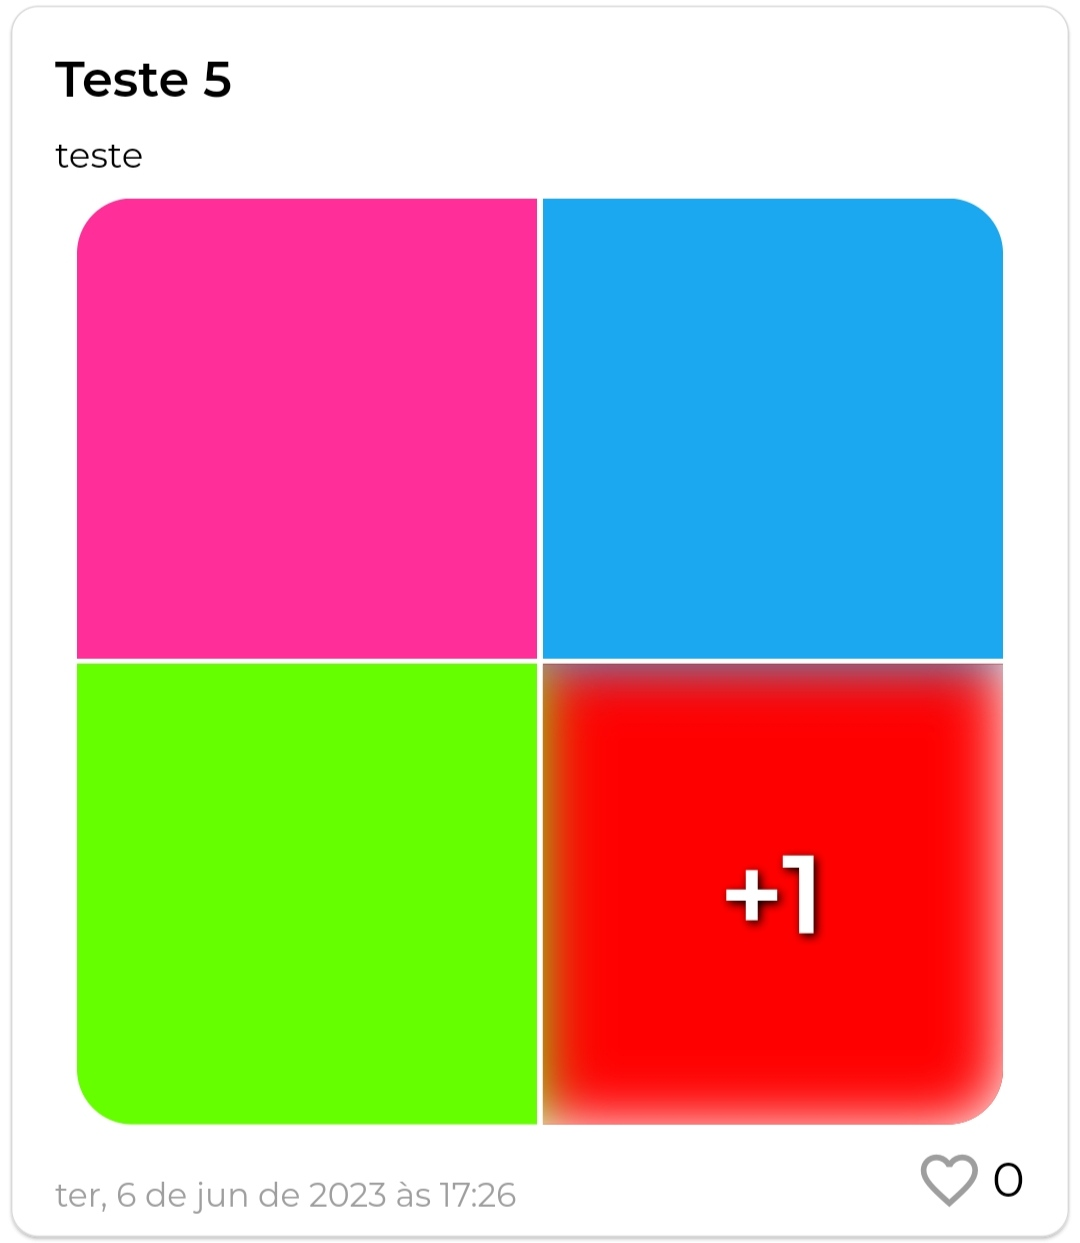
\includegraphics[width=0.2\textwidth]{images/implementacao/frontend/apresentacao_imagens/1686068843028.jpg} }}%
  \qquad
  \subfloat[\centering Publicação com 4 imagens]{{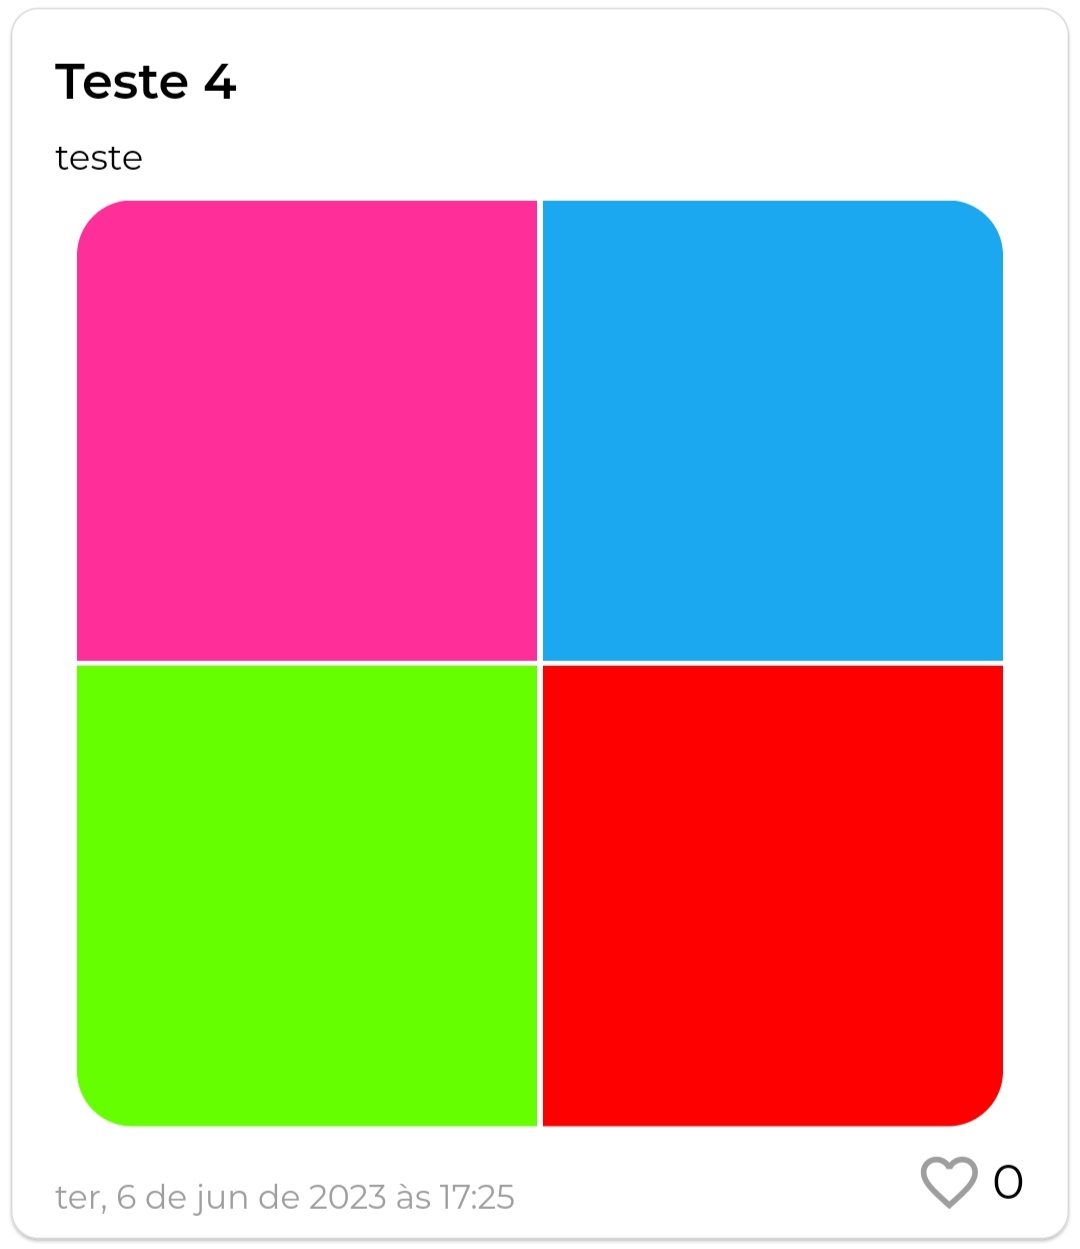
\includegraphics[width=0.2\textwidth]{images/implementacao/frontend/apresentacao_imagens/1686068843039.jpg} }}%
  \qquad
  \subfloat[\centering Publicação com 3 imagens]{{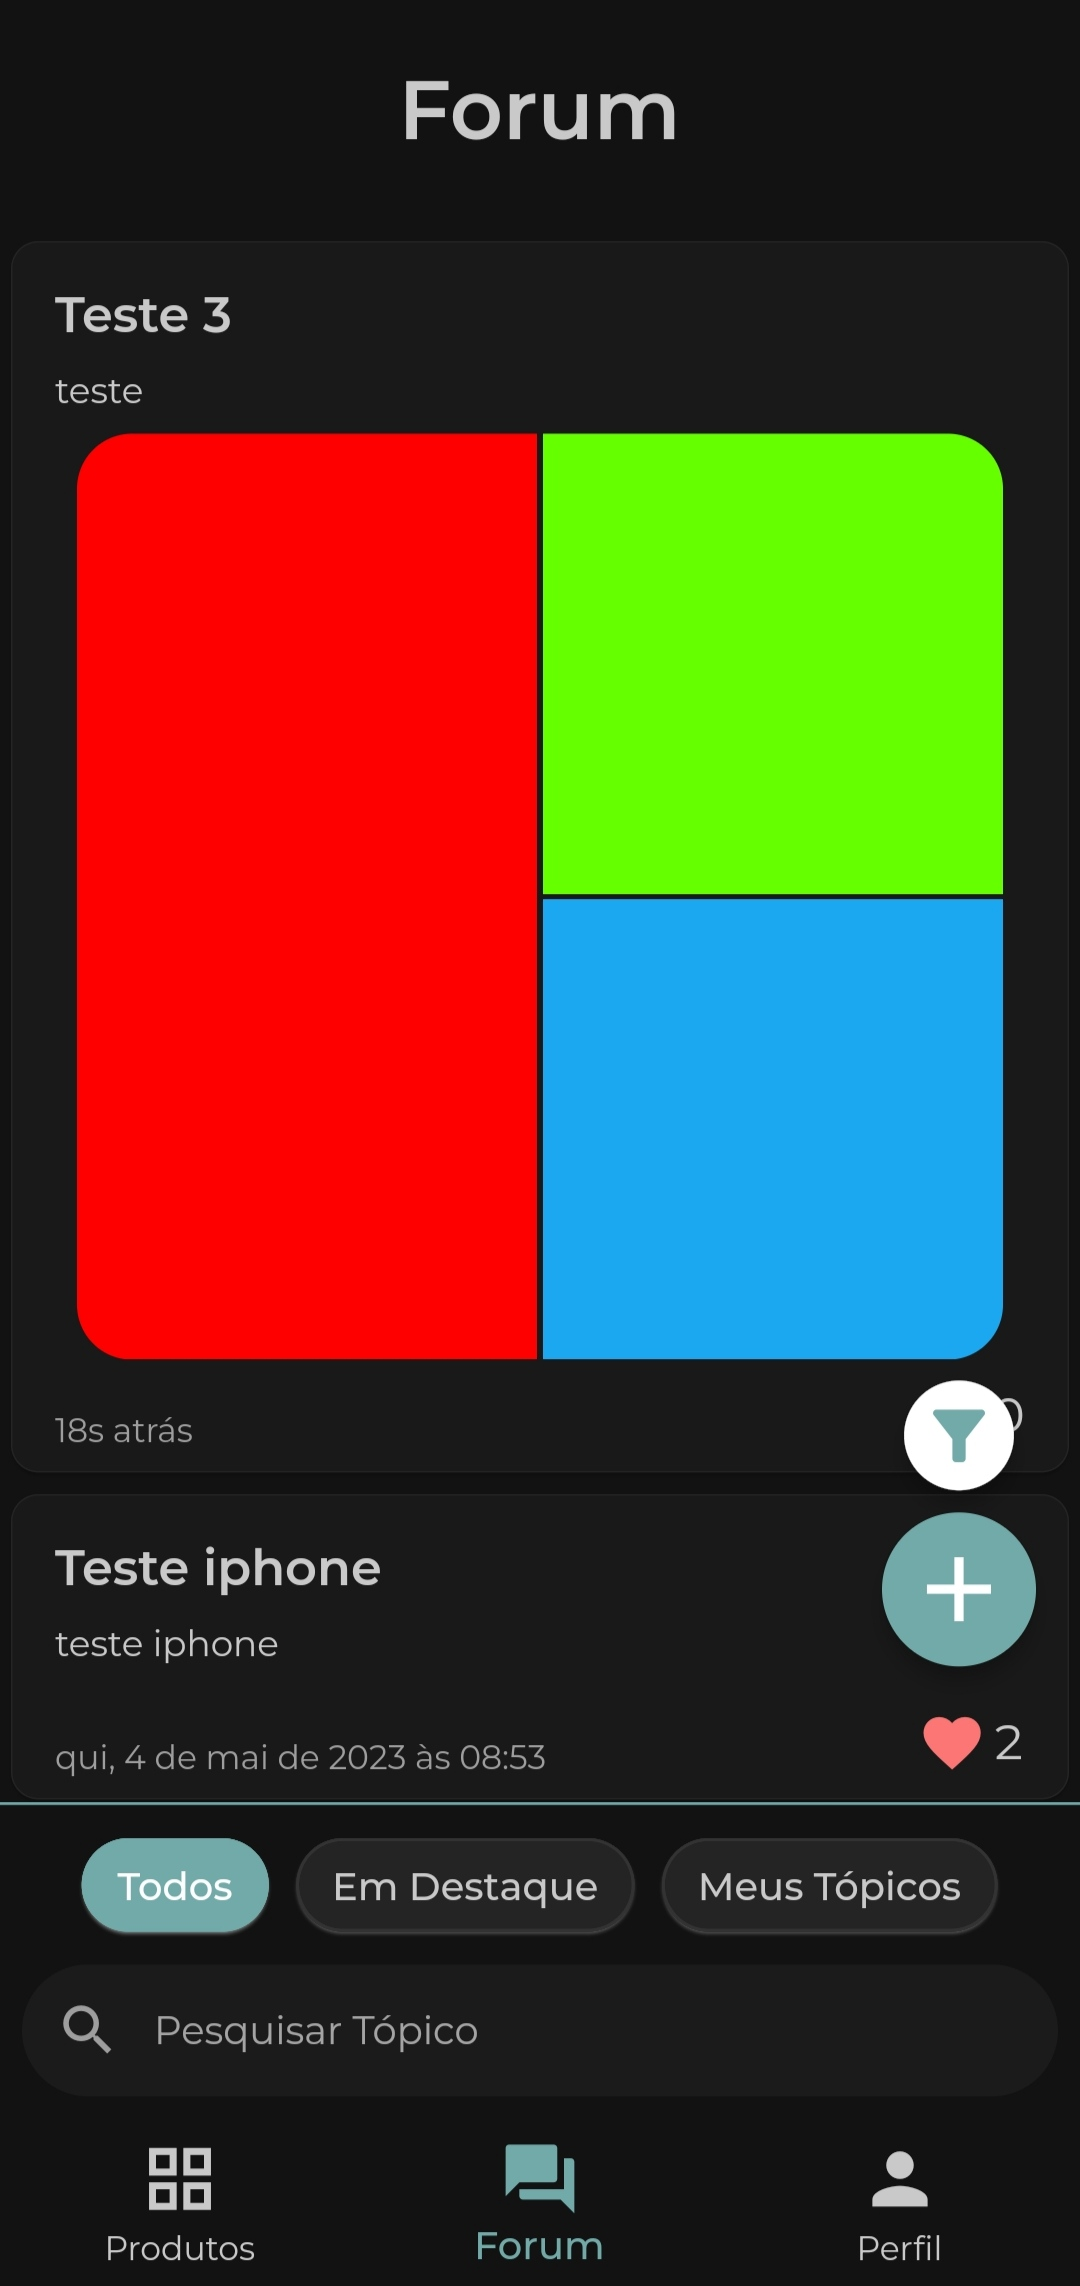
\includegraphics[width=0.2\textwidth]{images/implementacao/frontend/apresentacao_imagens/1686068843051.jpg} }}%
  \label{fig:76}%
\end{figure}

\newpage

\subsection{Apresentação de Imagens em carrosel}

A apresentação de imagens deverá permitir que o utilizador as visualize em ponto grande conseguindo também realizar diversas ações sobre estas, para isso foram experimentadas diversas bibliotecas, mas nunca se conseguia o comportamento desejado, sendo assim foi decidido criar o próprio carrosel de imagens, sendo que o próprio flutter já disponibiliza um widget para tal.

O ponto de maior dificuldade para este processo foi a implementação de zoom, visto que o flutter não dispõe de widgets para tal, sendo assim foi necessário primeiramente detetar gestos com o detetor de gestos da ferramenta e aplicado um zoom sobre o centro do gesto, os gestos aceites foram o de pinça e o gesto de duplo clique.

O grande problema com esta solução é que visto que é permitido um scroll horizontal de imagens os gestos por vezes poderão não funcionar corretamente, principalmente o gesto de pinça que se efetuado na horizontal poderá resultar em scroll horizontal. Para resolver tal problema foi decidido que quando dois dedos são detetados no ecrã a navegação horizontal fica bloqueada e assim que estes são levantados, a navegação horizontal é ativada novamente.

\subsection{Carregamento de Imagens}

O carregamento de imagens do dispositivo poderá ser realizado por meio de seleção de imagens da galeria, para realizar este tipo de seleção primeiramente foi testada a biblioteca image\_picker, mas esta biblioteca utiliza o seletor de ficheiro do dispositivo, o problema é que este tipo de seleção permite também a seleção de ficheiros também o que faz com que seja necessário um conjunto de outras verificações para garantir que apenas as imagens são selecionadas o que levaria a uma possível perda de performance e perda de qualidade na experiencia de utilização do utilizador.

Sendo assim foi de seguida testada a biblioteca advance\_image\_picker, mas o problema desta biblioteca é que não permite selecionar vídeos, pelo que foi decidido experimentar a biblioteca wechat\_asset\_picker, esta biblioteca cria uma página de seleção de imagens própria para seleção de imagens e vídeos diretamente da galeria, esta permite indicar o limite máximo de seleção e os tipos de ficheiros que o utilizador poderá selecionar de forma a que apenas os tipos aceites são mostrados, acrescentando também que esta biblioteca permite visualizar a tipagem de cada ficheiro no próprio objeto, o único ponto desvantajoso é que não é possível traduzir o botão de confirmação de seleção.

Após a carregar os ficheiros para memória, estes são então enviados para o firestorage como mencionado anteriormente.